\section{Normalizzazione nel Contesto dei Database}

La \textbf{normalizzazione} è un processo fondamentale nella progettazione di database relazionali. Il suo scopo principale è organizzare i dati in modo da:
\begin{enumerate}
	\item \textbf{Ridurre la ridondanza:} Evitare di ripetere le stesse informazioni in più punti.
	\item \textbf{Eliminare le anomalie:} Prevenire problemi che possono sorgere durante l'inserimento, l'aggiornamento o la cancellazione dei dati.
	\item \textbf{Garantire la qualità e l'integrità dei dati:} Assicurare che i dati siano coerenti e affidabili.
\end{enumerate}

Le \textbf{Forme Normali (FN)} sono un insieme di regole che definiscono quanto "ben formata" è una tabella (relazione). Se una relazione non è in una forma normale adeguata, può presentare:
\begin{itemize}
	\item \textbf{Ridondanze:} Dati duplicati inutilmente.
	\item \textbf{Comportamenti indesiderati durante gli aggiornamenti:} Ad esempio, la necessità di modificare lo stesso dato in più righe, con il rischio di dimenticarne qualcuna e creare inconsistenza.
\end{itemize}

La normalizzazione è una \textbf{tecnica di verifica} del design del database, non una metodologia di progettazione da zero. Prima progetti lo schema (magari con un modello E-R), poi lo verifichi e lo affini con la normalizzazione.

\subsection{Esempio di Tabella con Anomalie}
Consideriamo una tabella che traccia impiegati, progetti a cui lavorano, i loro stipendi, il budget dei progetti e il loro ruolo nel progetto:

\begin{center}
	\begin{tabular}{lllll}
		\toprule
		\textbf{Employee} & \textbf{Wage} & \textbf{Project} & \textbf{Budget} & \textbf{Role} \\
		\midrule
		Jones    & 20   & Mars     & 2      & Technician \\
		Smith    & 35   & Jupiter  & 15     & Designer   \\
		Smith    & 35   & Venus    & 15     & Designer   \\
		Williams & 55   & Venus    & 15     & Chief      \\
		Williams & 55   & Jupiter  & 15     & Consultant \\
		Williams & 55   & Mars     & 2      & Consultant \\
		Brown    & 48   & Mars     & 2      & Chief      \\
		Brown    & 48   & Venus    & 15     & Designer   \\
		White    & 48   & Venus    & 15     & Designer   \\
		White    & 48   & Jupiter  & 15     & Director   \\
		\bottomrule
	\end{tabular}
\end{center}

Questa tabella presenta diversi problemi (anomalie):
\begin{enumerate}
	\item \textbf{Ridondanza:}
	\begin{itemize}
		\item Lo stipendio (\texttt{Wage}) di un impiegato (es. Smith, 35) è ripetuto per ogni progetto a cui lavora.
		\item Il budget (\texttt{Budget}) di un progetto (es. Jupiter, 15) è ripetuto per ogni impiegato che ci lavora.
	\end{itemize}
	\item \textbf{Anomalia di Aggiornamento (Update Anomaly):}
	\begin{itemize}
		\item Se lo stipendio di Smith cambia, dobbiamo aggiornarlo in \textit{tutte} le righe in cui Smith compare. Se ne dimentichiamo una, il database diventa inconsistente.
	\end{itemize}
	\item \textbf{Anomalia di Cancellazione (Deletion Anomaly):}
	\begin{itemize}
		\item Se Jones smette di lavorare al progetto Mars (e Mars era il suo unico progetto), cancellando quella riga potremmo perdere l'informazione che Jones ha uno stipendio di 20 (se non ci sono altre tabelle che lo tracciano).
		\item Similmente, se il progetto Mars viene cancellato e Jones e Brown lavoravano solo a Mars, perderemmo le informazioni su Jones e Brown.
	\end{itemize}
	\item \textbf{Anomalia di Inserimento (Insertion Anomaly):}
	\begin{itemize}
		\item Non possiamo inserire un nuovo impiegato con il suo stipendio se non è ancora assegnato a un progetto.
		\item Non possiamo inserire un nuovo progetto con il suo budget se nessun impiegato ci sta ancora lavorando.
	\end{itemize}
\end{enumerate}

\subsection{Perché questa situazione è indesiderabile?}
Perché stiamo mescolando diversi "concetti" o "pezzi di informazione" nella stessa tabella:
\begin{itemize}
	\item Informazioni sugli impiegati e i loro stipendi.
	\item Informazioni sui progetti e i loro budget.
	\item Informazioni sul ruolo di un impiegato \textit{all'interno di uno specifico progetto}.
\end{itemize}

\section{Dipendenze Funzionali (Functional Dependencies - FD)}
Per studiare e risolvere queste anomalie in modo sistematico, introduciamo il concetto di \textbf{Dipendenza Funzionale (FD)}.
Una FD è un vincolo di integrità che descrive una relazione tra attributi all'interno di una tabella.

\subsection{Definizione Formale}
Data una relazione $r$ con uno schema $R(X)$ (dove X è l'insieme di tutti gli attributi), e dati due sottoinsiemi non vuoti di attributi $Y$ e $Z$ (contenuti in X), esiste una dipendenza funzionale $Y \rightarrow Z$ (si legge "Y determina funzionalmente Z" o "Z dipende funzionalmente da Y") se e solo se:
\textit{Per ogni coppia di tuple (righe) $t_1$ e $t_2$ in $r$, se i valori degli attributi in $Y$ sono uguali in $t_1$ e $t_2$ (cioè $t_1[Y] = t_2[Y]$), allora anche i valori degli attributi in $Z$ devono essere uguali (cioè $t_1[Z] = t_2[Z]$).}

In parole povere: se conosci il valore di $Y$, puoi determinare \textit{univocamente} il valore di $Z$.

\subsection{Spiegazione in termini più semplici}
"Determinare funzionalmente" significa semplicemente che se conosci il valore di un attributo, puoi conoscere con certezza il valore di un altro attributo.

\subsubsection{Esempi dalla tabella precedente}
\begin{itemize}
	\item $\text{Employee} \rightarrow \text{Wage}$
	\item $\text{Project} \rightarrow \text{Budget}$
	\item $\{\text{Employee, Project}\} \rightarrow \text{Role}$
\end{itemize}

\subsubsection{Spiegazione}

\begin{itemize}
	\item $\text{Employee} \rightarrow \text{Wage}$ significa: "Se sai chi è l'impiegato, sai sicuramente quanto guadagna". Nella nostra tabella, ogni volta che appare "Smith", il salario è sempre "35", ogni volta che appare "Jones" il salario è sempre "20". Il nome dell'impiegato \textit{determina} univocamente il suo stipendio.
	
	\item $\text{Project} \rightarrow \text{Budget}$ significa: "Se sai qual è il progetto, sai sicuramente qual è il suo budget". Ogni volta che vedi "Mars" come progetto, il budget è sempre "2", ogni volta che vedi "Jupiter", il budget è sempre "15".
\end{itemize}

\subsection{FD Triviali e Non Triviali}
\begin{itemize}
	\item Una FD $Y \rightarrow A$ è \textbf{triviale} se $A \subseteq Y$ (es. $\{\text{Employee, Project}\} \rightarrow \text{Project}$). Sono sempre vere e poco utili.
	\item Una FD $Y \rightarrow A$ è \textbf{non triviale} se $A \not\subseteq Y$. Sono queste che ci interessano per la normalizzazione.
\end{itemize}

\subsubsection{Spiegazione semplice con esempi pratici}

\textbf{Dipendenza Funzionale Triviale} - In termini semplici, è come dire "se conosci qualcosa, allora conosci anche una parte di quel qualcosa". 

\begin{itemize}
	\item \textbf{Esempio pratico:} In una tabella SQL \texttt{Clienti(ID, Nome, Cognome, Email)}, la dipendenza funzionale \texttt{\{ID, Nome, Cognome\} → Nome} è triviale perché ovviamente se conosci l'insieme \{ID, Nome, Cognome\}, allora conosci anche il Nome (che è già incluso nell'insieme).
	
	\item \textbf{In SQL:} Se scrivi \texttt{SELECT Nome FROM Clienti WHERE ID = 123 AND Nome = 'Mario' AND Cognome = 'Rossi'}, è ovvio che otterrai 'Mario' come risultato, perché è nelle condizioni stesse della query.
\end{itemize}

\textbf{Dipendenza Funzionale Non Triviale} - Significa che conoscendo alcuni attributi, puoi determinare altri attributi che \textit{non} sono già contenuti nei primi.

\begin{itemize}
	\item \textbf{Esempio pratico:} Nella tabella \texttt{Clienti(ID, Nome, Cognome, Email)}, la dipendenza \texttt{ID → Nome} è non triviale perché il Nome non è parte dell'ID e non è ovvio che l'ID determini il Nome.
	
	\item \textbf{In SQL:} Se scrivi \texttt{SELECT Nome FROM Clienti WHERE ID = 123}, otterrai un nome specifico perché esiste una dipendenza funzionale dall'ID al Nome (supponendo che ID sia una chiave primaria).
\end{itemize}

\textbf{Perché le FD triviali non sono utili per la normalizzazione?} Perché non rivelano nulla di nuovo sulla struttura dei dati. Sono sempre vere per definizione e non causano anomalie. Le dipendenze non triviali, invece, possono causare anomalie se non trattate correttamente.

\subsection{Come le FD causano anomalie}
Le anomalie sorgono principalmente quando abbiamo FD $X \rightarrow Y$ dove $X$ \textbf{non è una superchiave} (o chiave candidata) della tabella.
\begin{itemize}
	\item $\text{Employee} \rightarrow \text{Wage}$: \texttt{Employee} da solo non è la chiave. Causa ridondanza.
	\item $\text{Project} \rightarrow \text{Budget}$: \texttt{Project} da solo non è la chiave. Causa ridondanza.
	\item $\{\text{Employee, Project}\} \rightarrow \text{Role}$: $\{\text{Employee, Project}\}$ è (probabilmente) la chiave primaria. Questa FD \textbf{non causa anomalie}.
\end{itemize}
Le anomalie sono quindi causate dalla presenza di informazioni eterogenee.

\section{Forma Normale di Boyce-Codd (BCNF)}
La BCNF è una delle forme normali più stringenti e desiderabili.

\subsection{Definizione}
Una relazione $r$ è in \textbf{BCNF} se, per ogni dipendenza funzionale non triviale $X \rightarrow Y$ definita su $r$:
\begin{itemize}
	\item $X$ è una \textbf{superchiave} di $r$.
\end{itemize}

Nella nostra tabella di esempio iniziale, non è in BCNF a causa di $\text{Employee} \rightarrow \text{Wage}$ e $\text{Project} \rightarrow \text{Budget}$.

\subsubsection{Spiegazione della violazione BCNF}
Ricordiamo la definizione di BCNF: per ogni dipendenza funzionale non triviale $X \rightarrow Y$, $X$ deve essere una superchiave della relazione.

Nel nostro esempio:
\begin{itemize}
	\item $\text{Employee} \rightarrow \text{Wage}$: L'attributo \texttt{Employee} determina funzionalmente \texttt{Wage}. Ma \texttt{Employee} da solo non è una superchiave della tabella, perché non può determinare univocamente tutti gli altri attributi (come \texttt{Project}, \texttt{Budget}, \texttt{Role}). La chiave primaria della tabella è $\{\text{Employee, Project}\}$.
	\item $\text{Project} \rightarrow \text{Budget}$: Similmente, \texttt{Project} determina \texttt{Budget}, ma \texttt{Project} da solo non è una superchiave della tabella.
\end{itemize}

Queste violazioni causano le anomalie di inserimento, cancellazione e aggiornamento che abbiamo descritto in precedenza.

\textbf{Perché questo viola BCNF?} Perché BCNF richiede che quando un attributo (o gruppo di attributi) determina funzionalmente un altro attributo, il primo deve essere una "superchiave". In termini semplici, una superchiave è un attributo (o gruppo di attributi) che può identificare univocamente ogni riga nella tabella.

\subsection{Cosa fare se una relazione non è in BCNF?}
Si \textbf{decompone} la relazione in più relazioni più piccole, ognuna delle quali sia in BCNF.

\begin{center}
\begin{tikzpicture}[
	node distance=1cm and 0.8cm,
	box/.style={rectangle, rounded corners, draw, fill=black!80, minimum width=3.5cm, minimum height=1.2cm, align=center, text width=3.5cm},
	arrow/.style={->, >=stealth, thick}
]
% Step 1
\node[box] (start) {Relazione $R$ \\ non in BCNF};

% Step 2
\node[box, below=of start] (identify) {Identificare FD $X \rightarrow Y$ \\ che viola BCNF};

% Step 3
\node[box, below=of identify] (decompose) {Decomporre $R$ in \\ $R_1(X \cup Y)$ e $R_2(Z - (Y - X))$};

% Step 4
\node[box, below=of decompose] (check) {Verificare se $R_1$ e $R_2$ \\ sono in BCNF};

% Two branches
\node[box, below left=of check] (done) {Le relazioni \\ sono in BCNF};
\node[box, below right=of check] (repeat) {Ripetere};

% Arrows
\draw[arrow] (start) -- (identify);
\draw[arrow] (identify) -- (decompose);
\draw[arrow] (decompose) -- (check);
\draw[arrow] (check) -- node[above left, align=center] {Sì} (done);
\draw[arrow] (check) -- node[above right, align=center] {No} (repeat);
\draw[arrow] (repeat) to[out=180, in=0] (identify);
\end{tikzpicture}
\end{center}

\subsubsection{Esempio pratico di decomposizione}

\begin{minted}{text}
Esami(Matricola, Corso, Docente, Voto, Aula, Edificio)
↓ FDs che violano BCNF:
* Corso → Docente     (Corso non è superchiave)
* Aula → Edificio     (Aula non è superchiave)
\end{minted}

\noindent\textbf{Decomposizione in BCNF:}

\begin{center}
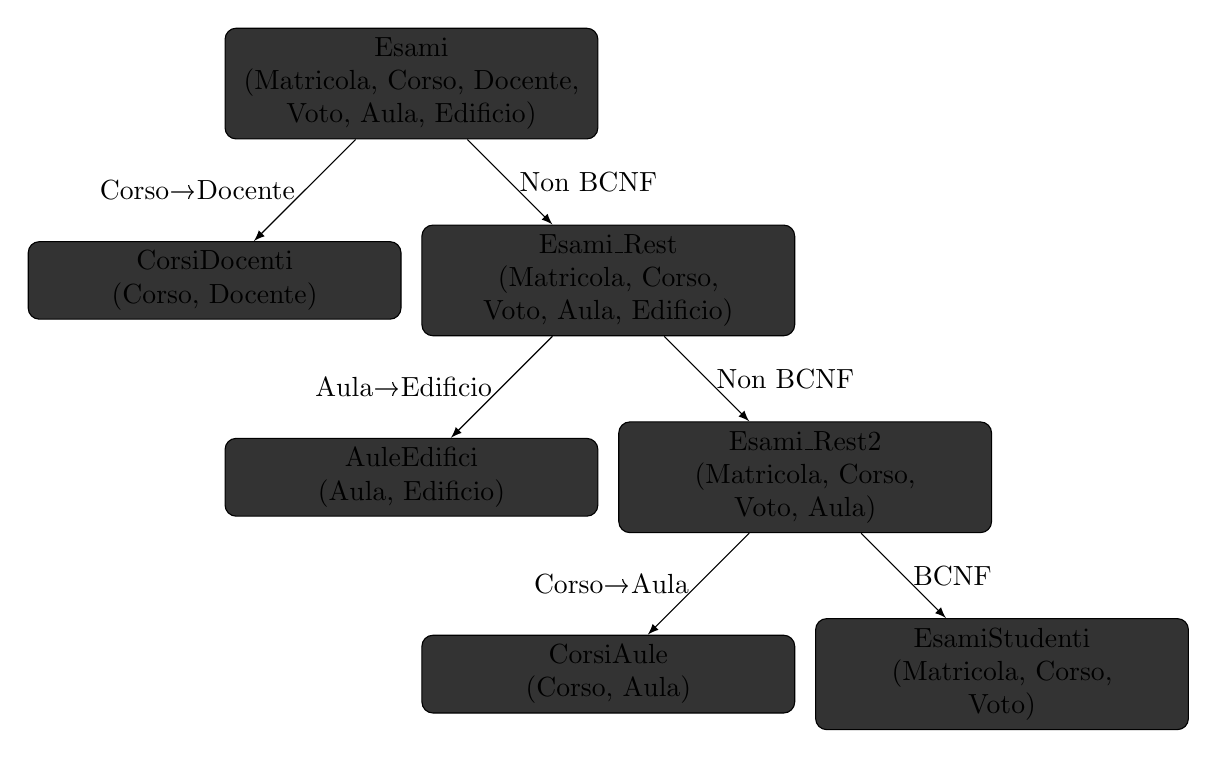
\begin{tikzpicture}[
	level distance=2.5cm,
	sibling distance=5cm,
	edge from parent/.style={draw, -latex},
	box/.style={rectangle, rounded corners, draw, fill=black!80, text width=4.5cm, align=center}
]
\node[box] {Esami\\(Matricola, Corso, Docente, \\Voto, Aula, Edificio)}
child {
	node[box] {CorsiDocenti\\(Corso, Docente)}
	edge from parent node[left, align=center] {Corso→Docente}
}
child {
	node[box] {Esami\_Rest\\(Matricola, Corso, \\Voto, Aula, Edificio)}
	child {
		node[box] {AuleEdifici\\(Aula, Edificio)}
		edge from parent node[left, align=center] {Aula→Edificio}
	}
	child {
		node[box] {Esami\_Rest2\\(Matricola, Corso, \\Voto, Aula)}
		child {
			node[box] {CorsiAule\\(Corso, Aula)}
			edge from parent node[left, align=center] {Corso→Aula}
		}
		child {
			node[box] {EsamiStudenti\\(Matricola, Corso, \\Voto)}
			edge from parent node[right, align=center] {BCNF}
		}
		edge from parent node[right, align=center] {Non BCNF}
	}
	edge from parent node[right, align=center] {Non BCNF}
};
\end{tikzpicture}
\end{center}

\subsubsection{Esempio con dipendenze più complesse}

\begin{minted}{text}
OrdiniFornitori(IDOrdine, CodiceArticolo, QuantitàOrdinata,
CodiceFornitore, RagioneSocialeFornitore, CittàFornitore)
FDs:
• IDOrdine → CodiceFornitore
• {IDOrdine, CodiceArticolo} → QuantitàOrdinata     (chiave)
• CodiceFornitore → {RagioneSocialeFornitore, CittàFornitore}
\end{minted}

\begin{center}
\begin{tabular}{|c|c|c|}
	\hline
	% \rowcolor{gray!30}
	\textbf{Ordini} & \textbf{Fornitori} & \textbf{DettagliOrdine} \\
	\hline
	\underline{IDOrdine} & \underline{CodiceFornitore} & \underline{IDOrdine, CodiceArticolo} \\
	CodiceFornitore & RagioneSocialeFornitore & QuantitàOrdinata \\
	& CittàFornitore & \\
	\hline
\end{tabular}
\end{center}

\subsection{Esempio di Decomposizione (per la tabella iniziale)}
\begin{enumerate}
	\item \textbf{ImpiegatiStipendi}(\underline{Employee}, Wage)
	\item \textbf{ProgettiBudget}(\underline{Project}, Budget)
	\item \textbf{ImpiegatiRuoliProgetto}(\underline{Employee, Project}, Role)
\end{enumerate}
Questa decomposizione elimina le anomalie.

\subsection{Qualità della Decomposizione}
Quando decomponiamo una tabella, dobbiamo assicurarci due proprietà fondamentali:

\subsubsection{Lossless Join Property (Proprietà di Join Senza Perdita)}
Dobbiamo essere in grado di ricreare la tabella originale facendo il JOIN delle tabelle decomposte.
\textbf{Condizione:} Una decomposizione di $r(X)$ in $r_1(X_1)$ e $r_2(X_2)$ è senza perdita se l'intersezione degli attributi $X_0 = X_1 \cap X_2$ forma una chiave per almeno una delle relazioni decomposte ($X_0 \rightarrow X_1$ oppure $X_0 \rightarrow X_2$).\

\textbf{Esempio di Decomposizione CON PERDITA:}
Supponiamo $R(\text{Employee, Project, Office})$ con FD: $\text{Employee} \rightarrow \text{Office}$ e $\text{Project} \rightarrow \text{Office}$.
Decomposizione in:
\begin{itemize}
	\item $R_1(\text{Employee, Office})$
	\item $R_2(\text{Project, Office})$
\end{itemize}

\noindent Tabella originale:
\begin{center}
\begin{tabular}{|l|l|l|}
	\hline
	\textbf{Employee} & \textbf{Project} & \textbf{Office} \\ \hline
	Smith & Alpha & A101 \\ \hline
	Jones & Beta & B202 \\ \hline
	Brown & Alpha & C303 \\ \hline
\end{tabular}
\end{center}

\noindent Tabelle decomposte:
\begin{center}
\begin{tabular}{|l|l|}
	\hline
	\textbf{Employee} & \textbf{Office} \\ \hline
	Smith & A101 \\ \hline
	Jones & B202 \\ \hline
	Brown & C303 \\ \hline
\end{tabular}
\quad
\begin{tabular}{|l|l|}
	\hline
	\textbf{Project} & \textbf{Office} \\ \hline
	Alpha & A101 \\ \hline
	Beta & B202 \\ \hline
	Alpha & C303 \\ \hline
\end{tabular}
\end{center}

\noindent Risultato del JOIN (genera tuple spurie):
\begin{center}
\begin{tabular}{|l|l|l|c|}
	\hline
	\textbf{Employee} & \textbf{Project} & \textbf{Office} & \textbf{Tuple Spurie} \\ \hline
	Smith & Alpha & A101 & \\ \hline
	Jones & Beta & B202 & \\ \hline
	Brown & Alpha & C303 & \\ \hline
	Smith & Alpha & C303 & \checkmark \\ \hline
	Brown & Alpha & A101 & \checkmark \\ \hline
\end{tabular}
\end{center}

\noindent Attributo comune: \texttt{Office}. \texttt{Office} non è chiave né per $R_1$ né per $R_2$. Il join può generare tuple spurie.

\textbf{Esempio di Decomposizione SENZA PERDITA:}
Tabella $R(\text{Employee, Project, Office})$ con FD: $\text{Employee} \rightarrow \text{Office}$ e chiave primaria $\{\text{Employee, Project}\}$.
Decomposizione in:
\begin{itemize}
	\item $R_1(\text{\underline{Employee}}, \text{Office})$
	\item $R_2(\text{\underline{Employee, Project}})$
\end{itemize}

\noindent Tabella originale:
\begin{center}
\begin{tabular}{|l|l|l|}
	\hline
	\textbf{Employee} & \textbf{Project} & \textbf{Office} \\ \hline
	Smith & Alpha & A101 \\ \hline
	Smith & Beta & A101 \\ \hline
	Jones & Gamma & B202 \\ \hline
\end{tabular}
\end{center}

\noindent Tabelle decomposte:
\begin{center}
\begin{tabular}{|l|l|}
	\hline
	\textbf{Employee} & \textbf{Office} \\ \hline
	Smith & A101 \\ \hline
	Jones & B202 \\ \hline
\end{tabular}
\quad
\begin{tabular}{|l|l|}
	\hline
	\textbf{Employee} & \textbf{Project} \\ \hline
	Smith & Alpha \\ \hline
	Smith & Beta \\ \hline
	Jones & Gamma \\ \hline
\end{tabular}
\end{center}

\noindent Risultato del JOIN (senza tuple spurie):
\begin{center}
\begin{tabular}{|l|l|l|}
	\hline
	\textbf{Employee} & \textbf{Project} & \textbf{Office} \\ \hline
	Smith & Alpha & A101 \\ \hline
	Smith & Beta & A101 \\ \hline
	Jones & Gamma & B202 \\ \hline
\end{tabular}
\end{center}

\noindent Attributo comune: \texttt{Employee}. \texttt{Employee} è chiave per $R_1$. Lossless.

\subsubsection{Dependency Preservation (Conservazione delle Dipendenze)}
Tutte le dipendenze funzionali originali devono poter essere verificate esaminando una singola tabella nello schema decomposto.
\newline
\newline
\textbf{In parole semplici:} La proprietà di conservazione delle dipendenze garantisce che, dopo aver decomposto una tabella in più tabelle, ogni regola (dipendenza funzionale) della tabella originale possa essere verificata esaminando \textit{una sola} delle tabelle risultanti, senza dover eseguire join.

Se $F$ è l'insieme delle dipendenze funzionali su $R$, e $R$ viene decomposto in $R_1, R_2, \ldots, R_n$, allora:
\begin{itemize}
	\item Per ogni dipendenza $X \rightarrow Y$ in $F$, deve esistere almeno un $R_i$ tale che $X \cup Y \subseteq R_i$
	\item Se nessun $R_i$ contiene tutti gli attributi di una dipendenza, allora quella dipendenza non può essere verificata senza combinare più tabelle
\end{itemize}

\textbf{Perché è importante?} Senza la conservazione delle dipendenze:
\begin{itemize}
	\item Diventa difficile mantenere l'integrità dei dati
	\item Le operazioni di controllo richiedono join costosi
	\item L'efficienza del database ne risente significativamente
\end{itemize}

\noindent Esempio di Decomposizione che \textbf{NON} preserva le dipendenze:

$R(\text{Employee}, \text{Project}, \text{Office})$ con dipendenze:

\begin{itemize}
	\item $\text{Employee} \rightarrow \text{Office}$
	\item $\text{Project} \rightarrow \text{Office}$
\end{itemize}

\noindent Tabella originale R:
\begin{center}
\begin{tabular}{|l|l|l|}
	\hline
	\textbf{Employee} & \textbf{Project} & \textbf{Office} \\ \hline
	Jones & Mars & Rome \\ \hline
	Smith & Jupiter & Milan \\ \hline
	Smith & Venus & Milan \\ \hline
	White & Saturn & Milan \\ \hline
	White & Venus & Milan \\ \hline
	White & Mars & Milan \\ \hline
\end{tabular}
\end{center}

\noindent Decomposizione in $R_1(\text{Employee, Office})$ e $R_2(\text{Employee, Project})$:
\begin{center}
\begin{tabular}{|l|l|}
	\hline
	\textbf{Employee} & \textbf{Office} \\ \hline
	Jones & Rome \\ \hline
	Smith & Milan \\ \hline
	White & Milan \\ \hline
\end{tabular}
\quad
\begin{tabular}{|l|l|}
	\hline
	\textbf{Employee} & \textbf{Project} \\ \hline
	Jones & Mars \\ \hline
	Smith & Jupiter \\ \hline
	Smith & Venus \\ \hline
	White & Saturn \\ \hline
	White & Venus \\ \hline
	White & Mars \\ \hline
\end{tabular}
\end{center}

\noindent La FD $\text{Project} \rightarrow \text{Office}$ \textbf{non è preservata} perché:
\begin{itemize}
	\item In $R_1$ manca l'attributo Project, quindi non può verificare Project → Office
	\item In $R_2$ manca l'attributo Office, quindi non può verificare Project → Office
	\item Non esiste nessuna singola tabella in cui possiamo verificare questa dipendenza
\end{itemize}

\noindent \textbf{Una decomposizione alternativa che preserva le dipendenze:}

Per preservare tutte le dipendenze funzionali, possiamo decomporre $R$ in tre tabelle:
\begin{itemize}
	\item $R_1(\text{Employee, Office})$ - preserva $\text{Employee} \rightarrow \text{Office}$
	\item $R_2(\text{Project, Office})$ - preserva $\text{Project} \rightarrow \text{Office}$
	\item $R_3(\text{Employee, Project})$ - mantiene la relazione tra Employee e Project
\end{itemize}

\noindent Decomposizione che preserva le dipendenze:
\begin{center}
\begin{tabular}{|l|l|}
	\hline
	\textbf{Employee} & \textbf{Office} \\ \hline
	Jones & Rome \\ \hline
	Smith & Milan \\ \hline
	White & Milan \\ \hline
\end{tabular}
\quad
\begin{tabular}{|l|l|}
	\hline
	\textbf{Project} & \textbf{Office} \\ \hline
	Mars & Rome \\ \hline
	Jupiter & Milan \\ \hline
	Venus & Milan \\ \hline
	Saturn & Milan \\ \hline
\end{tabular}
\quad
\begin{tabular}{|l|l|}
	\hline
	\textbf{Employee} & \textbf{Project} \\ \hline
	Jones & Mars \\ \hline
	Smith & Jupiter \\ \hline
	Smith & Venus \\ \hline
	White & Saturn \\ \hline
	White & Venus \\ \hline
	White & Mars \\ \hline
\end{tabular}
\end{center}

\noindent Questa decomposizione preserva tutte le dipendenze, (perché ogni dipendenza funzionale $X \rightarrow Y$ è contenuta interamente in almeno una delle tabelle risultanti: $\text{Employee} \rightarrow \text{Office}$ è in $R_1$ e $\text{Project} \rightarrow \text{Office}$ è in $R_2$) ma purtroppo \textbf{non garantisce} la proprietà di join senza perdita (lossless join). Infatti, quando riuniamo le tre tabelle, potremmo generare tuple spurie (ad esempio, dal join otterremmo che White lavora a Mars con Office = Rome, mentre nella tabella originale White lavora a Mars ma con Office = Milan; oppure potremmo ottenere Smith lavora a Mars, che non esiste nella relazione originale).

\noindent Il trade-off tra "Dependency Preservation" e "Lossless Join" è uno dei motivi per cui è stata definita la Terza Forma Normale (3NF).

\section{Recap: Quello che abbiamo imparato finora}

Piccolo riassunto di quanto visto finora:

\begin{itemize}
	\item \textbf{Normalizzazione:} È un processo per organizzare i dati in un database in modo da evitare ridondanze e anomalie. Serve a verificare e migliorare uno schema già progettato, non a crearlo da zero.
	
	\item \textbf{Anomalie:} Sono problemi che possono verificarsi quando lo schema del database non è ben progettato:
	\begin{itemize}
		\item \textbf{Anomalia di inserimento:} Non posso inserire certi dati se non ho altri dati correlati.
		\item \textbf{Anomalia di cancellazione:} Cancellando alcuni dati perdo accidentalmente altre informazioni importanti.
		\item \textbf{Anomalia di aggiornamento:} Devo aggiornare lo stesso dato in più punti, rischiando inconsistenze.
	\end{itemize}
	
	\item \textbf{Dipendenze Funzionali (FD):} Sono vincoli che esprimono come un attributo (o set di attributi) determina univocamente un altro attributo. Esempio: \texttt{Codice\_Fiscale → Data\_Nascita, Comune\_Nascita} significa che conoscendo il CF posso determinare con certezza la data di nascita e il comune di nascita.
	
	\item \textbf{Forma Normale di Boyce-Codd (BCNF):} Una tabella è in BCNF se per ogni dipendenza funzionale X → Y, X deve essere una superchiave (cioè deve poter identificare univocamente ogni riga della tabella).
	
	\item \textbf{Decomposizione:} Quando una tabella non è in BCNF, la dividiamo in tabelle più piccole che siano in BCNF.
	
	\item \textbf{Proprietà della decomposizione:}
	\begin{itemize}
		\item \textbf{Lossless Join:} La decomposizione deve permettere di ricostruire la tabella originale senza generare tuple spurie. Garantita se l'intersezione degli attributi forma una chiave per almeno una delle tabelle.
		\begin{itemize}
			\item \textbf{Esempio:} Se decompongo \texttt{Studenti(Matricola, Nome, CorsoDiLaurea)} in \newline \texttt{Anagrafica(Matricola, Nome)} e \texttt{Iscrizione(Matricola, CorsoDiLaurea)}, l'attributo comune \texttt{Matricola} è chiave per entrambe, quindi il join sarà senza perdita.
		\end{itemize}
		\item \textbf{Dependency Preservation:} Le dipendenze funzionali originali devono essere verificabili nelle tabelle decomposte senza fare join.
		\begin{itemize}
			\item \textbf{Esempio:} Se ho la FD \texttt{Matricola → CorsoDiLaurea} nella tabella originale, dopo la decomposizione devo poterla verificare in una singola tabella, ovvero \texttt{Iscrizione}.
		\end{itemize}
	\end{itemize}
	
	\item \textbf{Il problema:} Non sempre è possibile ottenere una decomposizione che sia sia lossless che preservi tutte le dipendenze e sia in BCNF.
\end{itemize}

Questo è il motivo per cui ora introduciamo la Terza Forma Normale (3NF), che è un po' meno restrittiva della BCNF ma garantisce sempre una decomposizione che preserva le dipendenze e ha la proprietà di lossless join.

\section{Terza Forma Normale (3NF)}
La 3NF è una forma normale leggermente meno stringente della BCNF che permette sempre una decomposizione lossless e che preserva le dipendenze.

\subsection{Definizione}
Una relazione $r$ è in \textbf{3NF} se, per ogni dipendenza funzionale non triviale $X \rightarrow Y$ definita su $r$, almeno una delle seguenti condizioni è vera:
\begin{enumerate}
	\item $X$ è una \textbf{superchiave} di $r$ (condizione BCNF).
	\textbf{OPPURE}
	\item Ogni attributo in $Y$ è parte di \textbf{almeno una chiave candidata} di $r$ (cioè, ogni attributo in $Y$ è un "attributo primo").
\end{enumerate}

\subsection{BCNF vs 3NF}
\begin{itemize}
	\item BCNF è più restrittiva. Ogni relazione in BCNF è anche in 3NF.
	\item Una relazione in 3NF potrebbe non essere in BCNF.
	\item Si può sempre decomporre una relazione in 3NF in modo lossless e preservando le dipendenze.
	\item Se una relazione ha una sola chiave candidata, allora 3NF e BCNF sono equivalenti.
\end{itemize}

\subsection{Esempio 3NF (ma non BCNF)}
Consideriamo una tabella $R(\text{Chief, Project, Office})$.
Supponiamo di avere le seguenti Dipendenze Funzionali (FDs):
\begin{enumerate}
	\item $\{\text{Project, Office}\} \rightarrow \text{Chief}$ (questa è una chiave candidata)
	\item $\text{Chief} \rightarrow \text{Office}$
\end{enumerate}

\noindent Un'istanza di esempio della tabella $R$ potrebbe essere:
\begin{center}
	\begin{tabular}{lll}
		\toprule
		\textbf{Chief} & \textbf{Project} & \textbf{Office} \\
		\midrule
		Rossi   & Alpha    & Stanza101 \\
		Rossi   & Beta     & Stanza101 \\
		Verdi   & Gamma    & Stanza202 \\
		Bianchi & Alpha    & Stanza303 \\ % Aggiunta per mostrare che {Project, Office} è chiave
		\bottomrule
	\end{tabular}
\end{center}

\noindent Da questa tabella, osserviamo:
\begin{itemize}
	\item Per la FD $\{\text{Project, Office}\} \rightarrow \text{Chief}$:
	\begin{itemize}
		\item $(\text{Alpha, Stanza101}) \rightarrow \text{Rossi}$
		\item $(\text{Beta, Stanza101}) \rightarrow \text{Rossi}$
		\item $(\text{Gamma, Stanza202}) \rightarrow \text{Verdi}$
		\item $(\text{Alpha, Stanza303}) \rightarrow \text{Bianchi}$
	\end{itemize}
	La coppia $\{\text{Project, Office}\}$ identifica univocamente \texttt{Chief}, quindi è una chiave candidata.
	
	\item Per la FD $\text{Chief} \rightarrow \text{Office}$:
	\begin{itemize}
		\item $\text{Rossi} \rightarrow \text{Stanza101}$
		\item $\text{Verdi} \rightarrow \text{Stanza202}$
		\item $\text{Bianchi} \rightarrow \text{Stanza303}$
	\end{itemize}
	L'attributo \texttt{Chief} determina univocamente \texttt{Office}.
\end{itemize}

Analizziamo ora la FD $\text{Chief} \rightarrow \text{Office}$ rispetto alle forme normali:
\begin{itemize}
	\item \textbf{BCNF:} La FD $\text{Chief} \rightarrow \text{Office}$ viola la BCNF perché $\text{Chief}$ non è una superchiave. (Ad esempio, \texttt{Chief} da solo non determina \texttt{Project}: Rossi è associato sia al progetto Alpha che Beta). \textbf{Quindi, R NON è in BCNF.}
	\item \textbf{3NF:} Per la FD $\text{Chief} \rightarrow \text{Office}$:
	\begin{enumerate}
		\item $\text{Chief}$ non è una superchiave. (Condizione 1 non soddisfatta)
		\item MA, ogni attributo in $Y$ (che è $\{\text{Office}\}$ in questo caso) è parte di almeno una chiave candidata di $R$. L'attributo $\text{Office}$ è infatti parte della chiave candidata $\{\text{Project, Office}\}$. (Condizione 2 soddisfatta)
	\end{enumerate}
	Poiché la seconda condizione è soddisfatta, \textbf{la relazione R È in 3NF.}
\end{itemize}

\subsection{Algoritmo di Decomposizione in 3NF (Idea Generale)}
\begin{enumerate}
	\item Trova un insieme minimo di dipendenze funzionali (copertura canonica).
	\item Per ogni FD $X \rightarrow Y$ in questa copertura, crea una tabella con attributi $X \cup Y$.
	\item Se nessuna delle tabelle create contiene una chiave candidata della relazione originale, aggiungi un'ulteriore tabella contenente solo gli attributi di una chiave candidata originale.
\end{enumerate}

\begin{center}
\begin{tikzpicture}[
	node distance=1cm and 0.8cm,
	box/.style={rectangle, rounded corners, draw, fill=black!80, minimum width=3.5cm, minimum height=1.2cm, align=center, text width=3.5cm},
	arrow/.style={->, >=stealth, thick}
]
% Step 1
\node[box] (start) {Relazione $R$ \\ con FDs $F$ \\ (non in 3NF)};

% Step 2
\node[box, below=of start] (mincover) {1. Calcolare la \\ copertura canonica $F_c$ di $F$.};

% Step 3
\node[box, below=of mincover] (decomporre) {2. Per ogni FD $X \rightarrow Y$ in $F_c$, creare una relazione $R_i(X \cup Y)$.};

% Step 4
\node[box, below=of decomporre] (checkkey) {3. Verificare se una chiave candidata di $R$ è contenuta in una delle $R_i$.};

% Step 5a (Yes)
\node[box, below left=of checkkey, xshift=-1cm] (done) {Le relazioni $R_i$ \\ sono la decomposizione \\ in 3NF.};

% Step 5b (No)
\node[box, below right=of checkkey, xshift=1cm] (addkey) {Aggiungere una relazione $R_k$ contenente solo gli attributi di una chiave candidata di $R$. \\ Le $R_i \cup \{R_k\}$ sono la decomposizione in 3NF.};

% Arrows
\draw[arrow] (start) -- (mincover);
\draw[arrow] (mincover) -- (decomporre);
\draw[arrow] (decomporre) -- (checkkey);
\draw[arrow] (checkkey.west) -- node[above, pos=0.4, align=center] {Sì} (done.north);
\draw[arrow] (checkkey.east) -- node[above, pos=0.4, align=center] {No} (addkey.north);

\end{tikzpicture}
\end{center}

\subsection{Approccio Pratico Consigliato}
\begin{enumerate}
	\item Decomponi la relazione per raggiungere la 3NF.
	\item Verifica se le tabelle risultanti sono anche in BCNF.
	\item Se una tabella è in 3NF ma non in BCNF, valuta il trade-off.
\end{enumerate}

\subsection{Teoria delle Dipendenze e Implicazioni}
Dato un insieme di dipendenze funzionali $F$, possiamo derivare altre dipendenze funzionali. Diciamo che $F$ implica $f$ se ogni relazione che soddisfa $F$ soddisfa anche $f$. L'insieme di tutte le dipendenze implicite da $F$ è chiamato \textbf{chiusura di F ($F^+$)}.

\subsubsection{Assiomi di Armstrong}
\begin{enumerate}
	\item \textbf{Riflessività:} Se $Y \subseteq X$, allora $X \rightarrow Y$.
	\item \textbf{Aumento:} Se $X \rightarrow Y$, allora $XZ \rightarrow YZ$.
	\item \textbf{Transitività:} Se $X \rightarrow Y$ e $Y \rightarrow Z$, allora $X \rightarrow Z$.
	\begin{itemize}
		\item Esempio: $\text{MatricolaStudente} \rightarrow \text{CodiceCorsoLaurea}$ e $\text{CodiceCorsoLaurea} \rightarrow \text{NomeCorsoLaurea}$. Allora, $\text{MatricolaStudente} \rightarrow \text{NomeCorsoLaurea}$.
	\end{itemize}
\end{enumerate}

\subsubsection{Chiusura di un insieme di attributi $X^+$}
L'insieme di tutti gli attributi che sono funzionalmente determinati da X, dato un insieme di FDs F.

\subsubsection{Copertura Minima (o Canonica)}
Un insieme "minimale" di FDs equivalente a F, senza ridondanze.

\section{Normalizzazione nel Design Concettuale (Modello E-R)}
La teoria della normalizzazione può essere usata anche per verificare la qualità di un modello Entità-Relazione.

\subsection{Esempio: Normalizzazione su Entità}
Considera un'entità \texttt{Prodotto} con attributi:
\texttt{Codice} (PK), \texttt{NomeProdotto}, \texttt{Prezzo}, \texttt{PartitaIVAFornitore}, \texttt{NomeFornitore}, \texttt{IndirizzoFornitore}.

Identifichiamo una FD: $\text{PartitaIVAFornitore} \rightarrow \text{NomeFornitore, IndirizzoFornitore}$.
Qui, \texttt{PartitaIVAFornitore} non è la chiave di \texttt{Prodotto}.
Questo viola le forme normali.

\textbf{Decomposizione dell'Entità:}
\begin{itemize}
	\item Entità \texttt{Prodotto}(\underline{\texttt{Codice}}, \texttt{NomeProdotto}, \texttt{Prezzo})
	\item Entità \texttt{Fornitore}(\underline{\texttt{PartitaIVAFornitore}}, \texttt{NomeFornitore}, \texttt{IndirizzoFornitore})
	\item Relazione \texttt{Fornisce} tra \texttt{Fornitore} e \texttt{Prodotto}.
\end{itemize}
Nello schema proposto dalla slide 54:
\begin{itemize}
	\item \texttt{Product(Code, Name, Price)}
	\item \texttt{Supplier(VATNum, Name, Address)}
	\item \texttt{Supply} (relationship)
\end{itemize}

\subsection{Esempio: Normalizzazione su Relazioni (Relationship)}
Considera una relazione \texttt{Tesi} che collega \texttt{Studente}, \texttt{Professore}, \texttt{DipartimentoProf}, \texttt{CorsoLaureaStudente}.
Assumiamo che $(\text{MatricolaStudente, IDProfessore})$ sia la chiave.
FDs:
\begin{itemize}
	\item $\text{MatricolaStudente} \rightarrow \text{CorsoLaureaStudente}$
	\item $\text{IDProfessore} \rightarrow \text{DipartimentoProf}$
\end{itemize}
Nella tabella \texttt{Tesi}(\underline{MatricolaStudente, IDProfessore}, CorsoLaureaStudente, DipartimentoProf):
\begin{itemize}
	\item $\text{IDProfessore} \rightarrow \text{DipartimentoProf}$: \texttt{IDProfessore} è parte della chiave, non la chiave intera. \texttt{DipartimentoProf} non è un attributo primo. Viola 3NF/BCNF.
\end{itemize}

\textbf{Decomposizione della Relazione (Conceptual Level):}
\begin{enumerate}
	\item Creare un'entità \texttt{Professore} con attributo \texttt{Dipartimento} (slide 50: \texttt{Professor --(1,1)-- Work --(0,N)-- Dept}).
	\item Creare un'entità \texttt{Studente} con attributo \texttt{CorsoLaurea} (slide 52: \texttt{Student --(1,1)-- Enroll --(0,N)-- Degree}).
	\item La relazione \texttt{Tesi} ora collegherebbe solo \texttt{Studente} e \texttt{Professore} (slide 52: \texttt{Professor --(0,N)-- Thesis --(0,1)-- Student}).
\end{enumerate}
Questo processo porta a un modello concettuale più robusto.

